% -----------------------------------------------------------------------------
% The MIT License (MIT)
%
% Copyright (c) 2015 Pejman Ghorbanzade
%
% Permission is hereby granted, free of charge, to any person obtaining a copy
% of this software and associated documentation files (the "Software"), to deal
% in the Software without restriction, including without limitation the rights
% to use, copy, modify, merge, publish, distribute, sublicense, and/or sell
% copies of the Software, and to permit persons to whom the Software is
% furnished to do so, subject to the following conditions:
%
% The above copyright notice and this permission notice shall be included in
% all copies or substantial portions of the Software.
%
% THE SOFTWARE IS PROVIDED "AS IS", WITHOUT WARRANTY OF ANY KIND, EXPRESS OR
% IMPLIED, INCLUDING BUT NOT LIMITED TO THE WARRANTIES OF MERCHANTABILITY,
% FITNESS FOR A PARTICULAR PURPOSE AND NONINFRINGEMENT. IN NO EVENT SHALL THE
% AUTHORS OR COPYRIGHT HOLDERS BE LIABLE FOR ANY CLAIM, DAMAGES OR OTHER
% LIABILITY, WHETHER IN AN ACTION OF CONTRACT, TORT OR OTHERWISE, ARISING FROM,
% OUT OF OR IN CONNECTION WITH THE SOFTWARE OR THE USE OR OTHER DEALINGS IN
% THE SOFTWARE.
% -----------------------------------------------------------------------------

\def \topDirectory {../..}

\documentclass[10pt, compress]{beamer}

\usepackage{\topDirectory/template/style/directives}
%%%%%%%%%%%%%%%%%%%%%%%%%%%%%%%%%%%%%%%%%%%%%%%%%%%%%%%%%%%%%%%%%%%%%%%%%%%%%%
% CS110: Introduction to Computing
% Copyright 2015 Pejman Ghorbanzade <mail@ghorbanzade.com>
% Creative Commons Attribution-ShareAlike 4.0 International License
% https://github.com/ghorbanzade/UMB-CS110-2015S/blob/master/LICENSE
%%%%%%%%%%%%%%%%%%%%%%%%%%%%%%%%%%%%%%%%%%%%%%%%%%%%%%%%%%%%%%%%%%%%%%%%%%%%%%

\course{id}{CS110}
\course{name}{Introduction to Computing}
\course{venue}{Tue/Thu, 5:30 PM - 6:45 PM}
\course{semester}{Spring 2015}
\course{department}{Department of Computer Science}
\course{university}{University of Massachusetts Boston}

\instructor{name}{Pejman Ghorbanzade}
\instructor{title}{}
\instructor{position}{Student Instructor}
\instructor{email}{pejman@cs.umb.edu}
\instructor{phone}{617-287-6419}
\instructor{office}{S-3-124B}
\instructor{office-hours}{Tue/Thu 19:00-20:30}
\instructor{address}{University of Massachusetts Boston, 100 Morrissey Blvd., Boston, MA}

\usepackage{\topDirectory/template/style/beamerthemeUmassLecture}
\doc{number}{2}
%\setbeamertemplate{footline}[text line]{}

\begin{document}
\prepareCover

\section{Course Administration}

\begin{frame}[fragile]
	\frametitle{Course Administration}
	\begin{itemize}
		\item[] 25/58 student accounts so far.
		\item[] Submit online questionnaire.
		\item[] Assignment 1 released. Due on Feb 17 at 5:30 PM. Submission online. No paper copies.
		\item[] Bring laptops for lectures and lab sessions.
	\end{itemize}
\end{frame}

\begin{frame}[fragile]
	\frametitle{Course Administration}
	\begin{block}{Overview}
		\begin{itemize}
			\item[] Computer Programming
			\item[] Programming Languages
			\item[] Java Programming Language
		\end{itemize}
	\end{block}
\end{frame}

\section{Computer Programming}

\begin{frame}[fragile]
	\frametitle{Computer Programming}
	\begin{block}{Philosophy}
		\begin{columns}
			\begin{column}{0.4\textwidth}
			\begin{itemize}
				\item[] Strong Points
				\begin{itemize}
					\item[] Fast computing
					\item[] No fatigue
				\end{itemize}
				\item[] Weak Points
				\begin{itemize}
					\item[] Hard to Teach
					\item[] No Innovation
				\end{itemize}
			\end{itemize}
			\end{column}
			\begin{column}{0.6\textwidth}
			\begin{figure}[H]\centering
				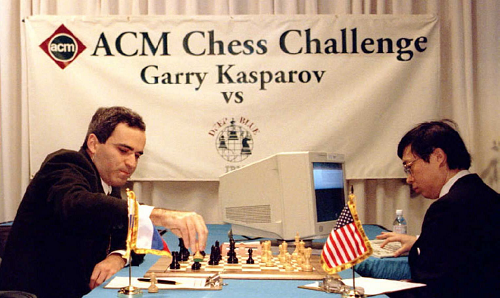
\includegraphics[width=\textwidth]{\topDirectory/template/images/chess.png}
			\end{figure}
			\end{column}
		\end{columns}
	\end{block}
\end{frame}

\begin{frame}[fragile]
	\frametitle{Computer Programming}
	\begin{block}{Computers are good at}
		\begin{itemize}
			\item[] Repetitive simple but tedious computations
			\item[] One-time long and complex computations
		\end{itemize}
	\end{block}
	\begin{block}{Motivation}
		To harvest computers power for solving everyday problems
	\end{block}
\end{frame}

\begin{frame}[fragile]
	\frametitle{Computer Programming}
	\begin{block}{Conflicts}
			\begin{itemize}
				\item[] Computers speak in zeros and ones.
				\item[] Humans speak in prose and verse.
			\end{itemize}
	\end{block}
	\begin{quote}
		Programming languages are efforts to develop a common language easy-to-understand for both.
	\end{quote}
\end{frame}

\begin{frame}[fragile]
	\frametitle{Computer Programming}
	\begin{block}{It's all about thinking}
		\begin{quote}
		``Instead of imagining that our main task is to instruct a computer what to do, let us concentrate rather on explaining to human beings what we want a computer to do.''
		\begin{flushright}
		- Donald Knuth
		\end{flushright}
		\end{quote}
	\end{block}
\end{frame}

\section{Programming Languages}

\begin{frame}[fragile]
	\frametitle{Programming Languages}
	\begin{block}{Classification}
		\begin{columns}
			\begin{column}{0.5\textwidth}
			\begin{itemize}
				\item[] By level of abstraction
				\begin{itemize}
					\item[] Low-level languages
					\item[] High-level languages
					\item[] Very-high-level languages
					\item[]
				\end{itemize}
			\end{itemize}
			\end{column}
			\begin{column}{0.5\textwidth}
			\begin{itemize}
				\item[] By method of execution
				\begin{itemize}
					\item[] Machine Code
					\item[] Assembler
					\item[] Compiler
					\item[] Interpreter
				\end{itemize}
			\end{itemize}
			\end{column}
		\end{columns}
	\end{block}
\end{frame}

\begin{frame}[fragile]
	\frametitle{Programming Languages}
	\begin{block}{A Closer Look}
		\begin{figure}\centering
			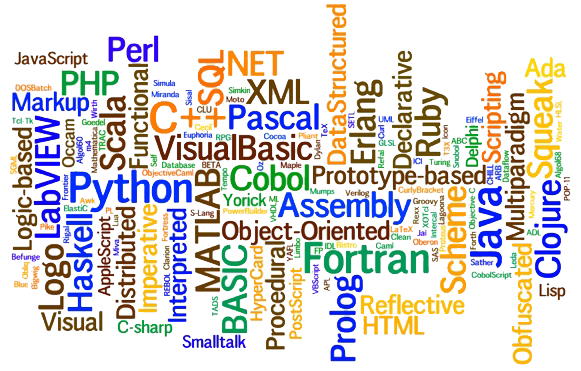
\includegraphics[width=\textwidth]{\topDirectory/template/images/languages.png}
		\end{figure}
	\end{block}
\end{frame}

\begin{frame}[fragile]
	\frametitle{Programming Languages}
	\begin{block}{A Closer Look}
		Let's taste some code!
		\begin{columns}
			\begin{column}{0.5\textwidth}
			\begin{itemize}
				\item[] Machine Language
				\item[] Assembly
				\item[] C
				\item[] C++
				\item[] Python
			\end{itemize}
			\end{column}
			\begin{column}{0.5\textwidth}
			\begin{itemize}
				\item[] Perl
				\item[] Ruby
				\item[] Matlab
				\item[] LabVIEW
				\item[] Scratch
			\end{itemize}
			\end{column}
		\end{columns}
	\end{block}
\end{frame}

\section{Java Programming Language}

\begin{frame}[fragile]
	\frametitle{Java Programming Language}
	\begin{block}{Goals}
		\begin{columns}
			\begin{column}{0.7\textwidth}
			\begin{itemize}
				\item[] To be simple, object-oriented and familiar
				\item[] To be robust and secure
				\item[] To be architecture-neutral and portable
				\item[] To execute with high performance
				\item[] To be interpreted, threaded and dynamic
			\end{itemize}
			\end{column}
			\begin{column}{0.3\textwidth}
			\begin{figure}
				
\includegraphics[width=\textwidth]{\topDirectory/template/images/logo.png}
			\end{figure}
			\end{column}
		\end{columns}
	\end{block}
\end{frame}

\begin{frame}[fragile]
	\frametitle{Java Programming Language}
	\begin{block}{Execution Procedure}
		\begin{itemize}
			\item[] Java code is compiled to Java Bytecode
			\item[] Java bytecode is interpreted by Java Virtual Machine
			\item[] Java Virtual Machine converts Java Bytecode to machine code.
			\item[] Sacrifice speed to achieve portability
		\end{itemize}
	\end{block}
\end{frame}

\begin{frame}[fragile]
	\frametitle{Java Programming Language}
	\begin{block}{Applications}
		\begin{itemize}
			\item[] Java Applets
			\item[] Java Servlets
			\item[] Java Server Pages
			\item[] Java Database Connectivity
		\end{itemize}
	\end{block}
\end{frame}

\begin{frame}[fragile]
	\frametitle{Java Programming Language}
	\begin{block}{HelloWorld.java}
		\begin{minted}[fontsize=\small, linenos, firstnumber=1]{java}
public class HelloWorld {
	public static void main(String[] args) {
		System.out.println("Hello CS110 Students!");
	}
}
		\end{minted}
	\end{block}
\end{frame}

\plain{}{Keep Calm\\and\\Code}

\end{document}
